\section{Конструкторская часть}

% В данном разделе будет проведён анализ существующих операционных систем для устройств интернета вещей. Рассматриваемые операционные системы будут относиться к одному из двух типов: ОС реального времени и ОС разделения времени.

\subsection{Проектирование БД}

\subsubsection{Формализация сущностей системы}

На рисунке \ref{fig:db} представлена диаграмма, отражающая информацию о таблицах проектируемой БД.

\begin{figure}[h]
	\centering
	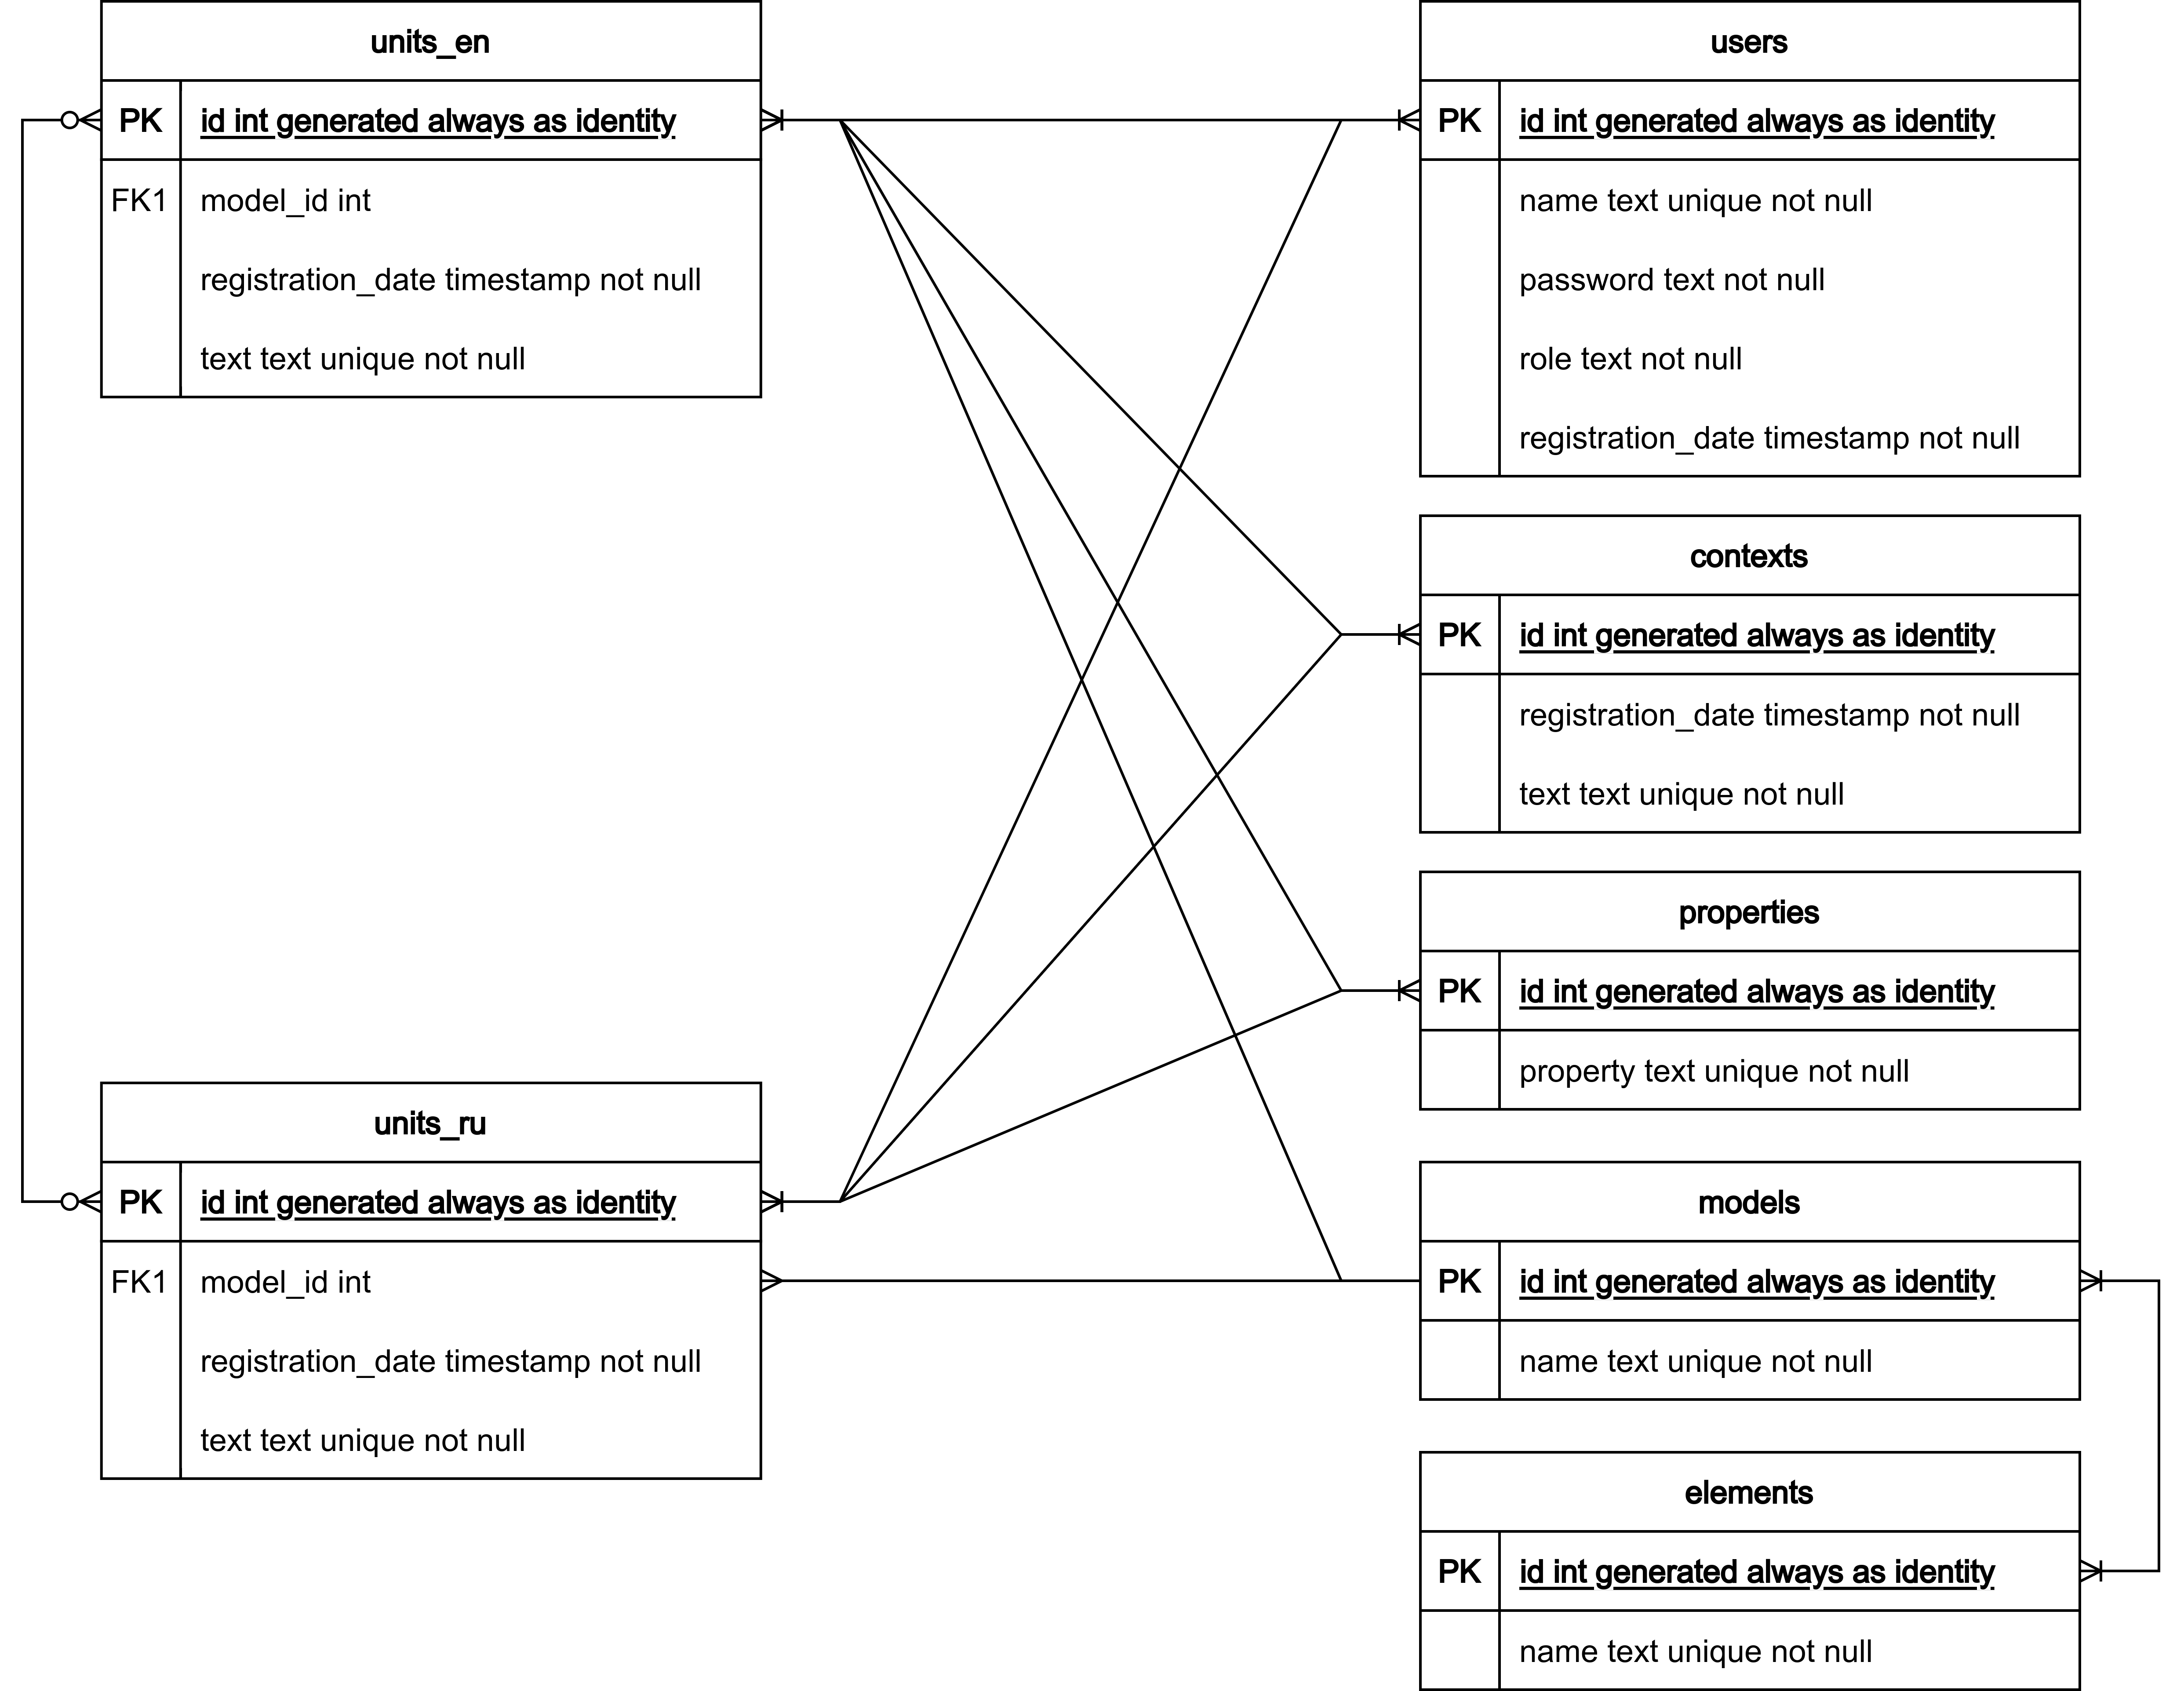
\includegraphics[width=\textwidth ]{img/db/db.drawio.png}
	\caption{Диаграмма базы данных}
	\label{fig:db}
\end{figure} 

\subsubsection{Хранимые процедуры БД}

Описать, какие процедуры нужны и зачем.

\begin{figure}[h]
	\centering
	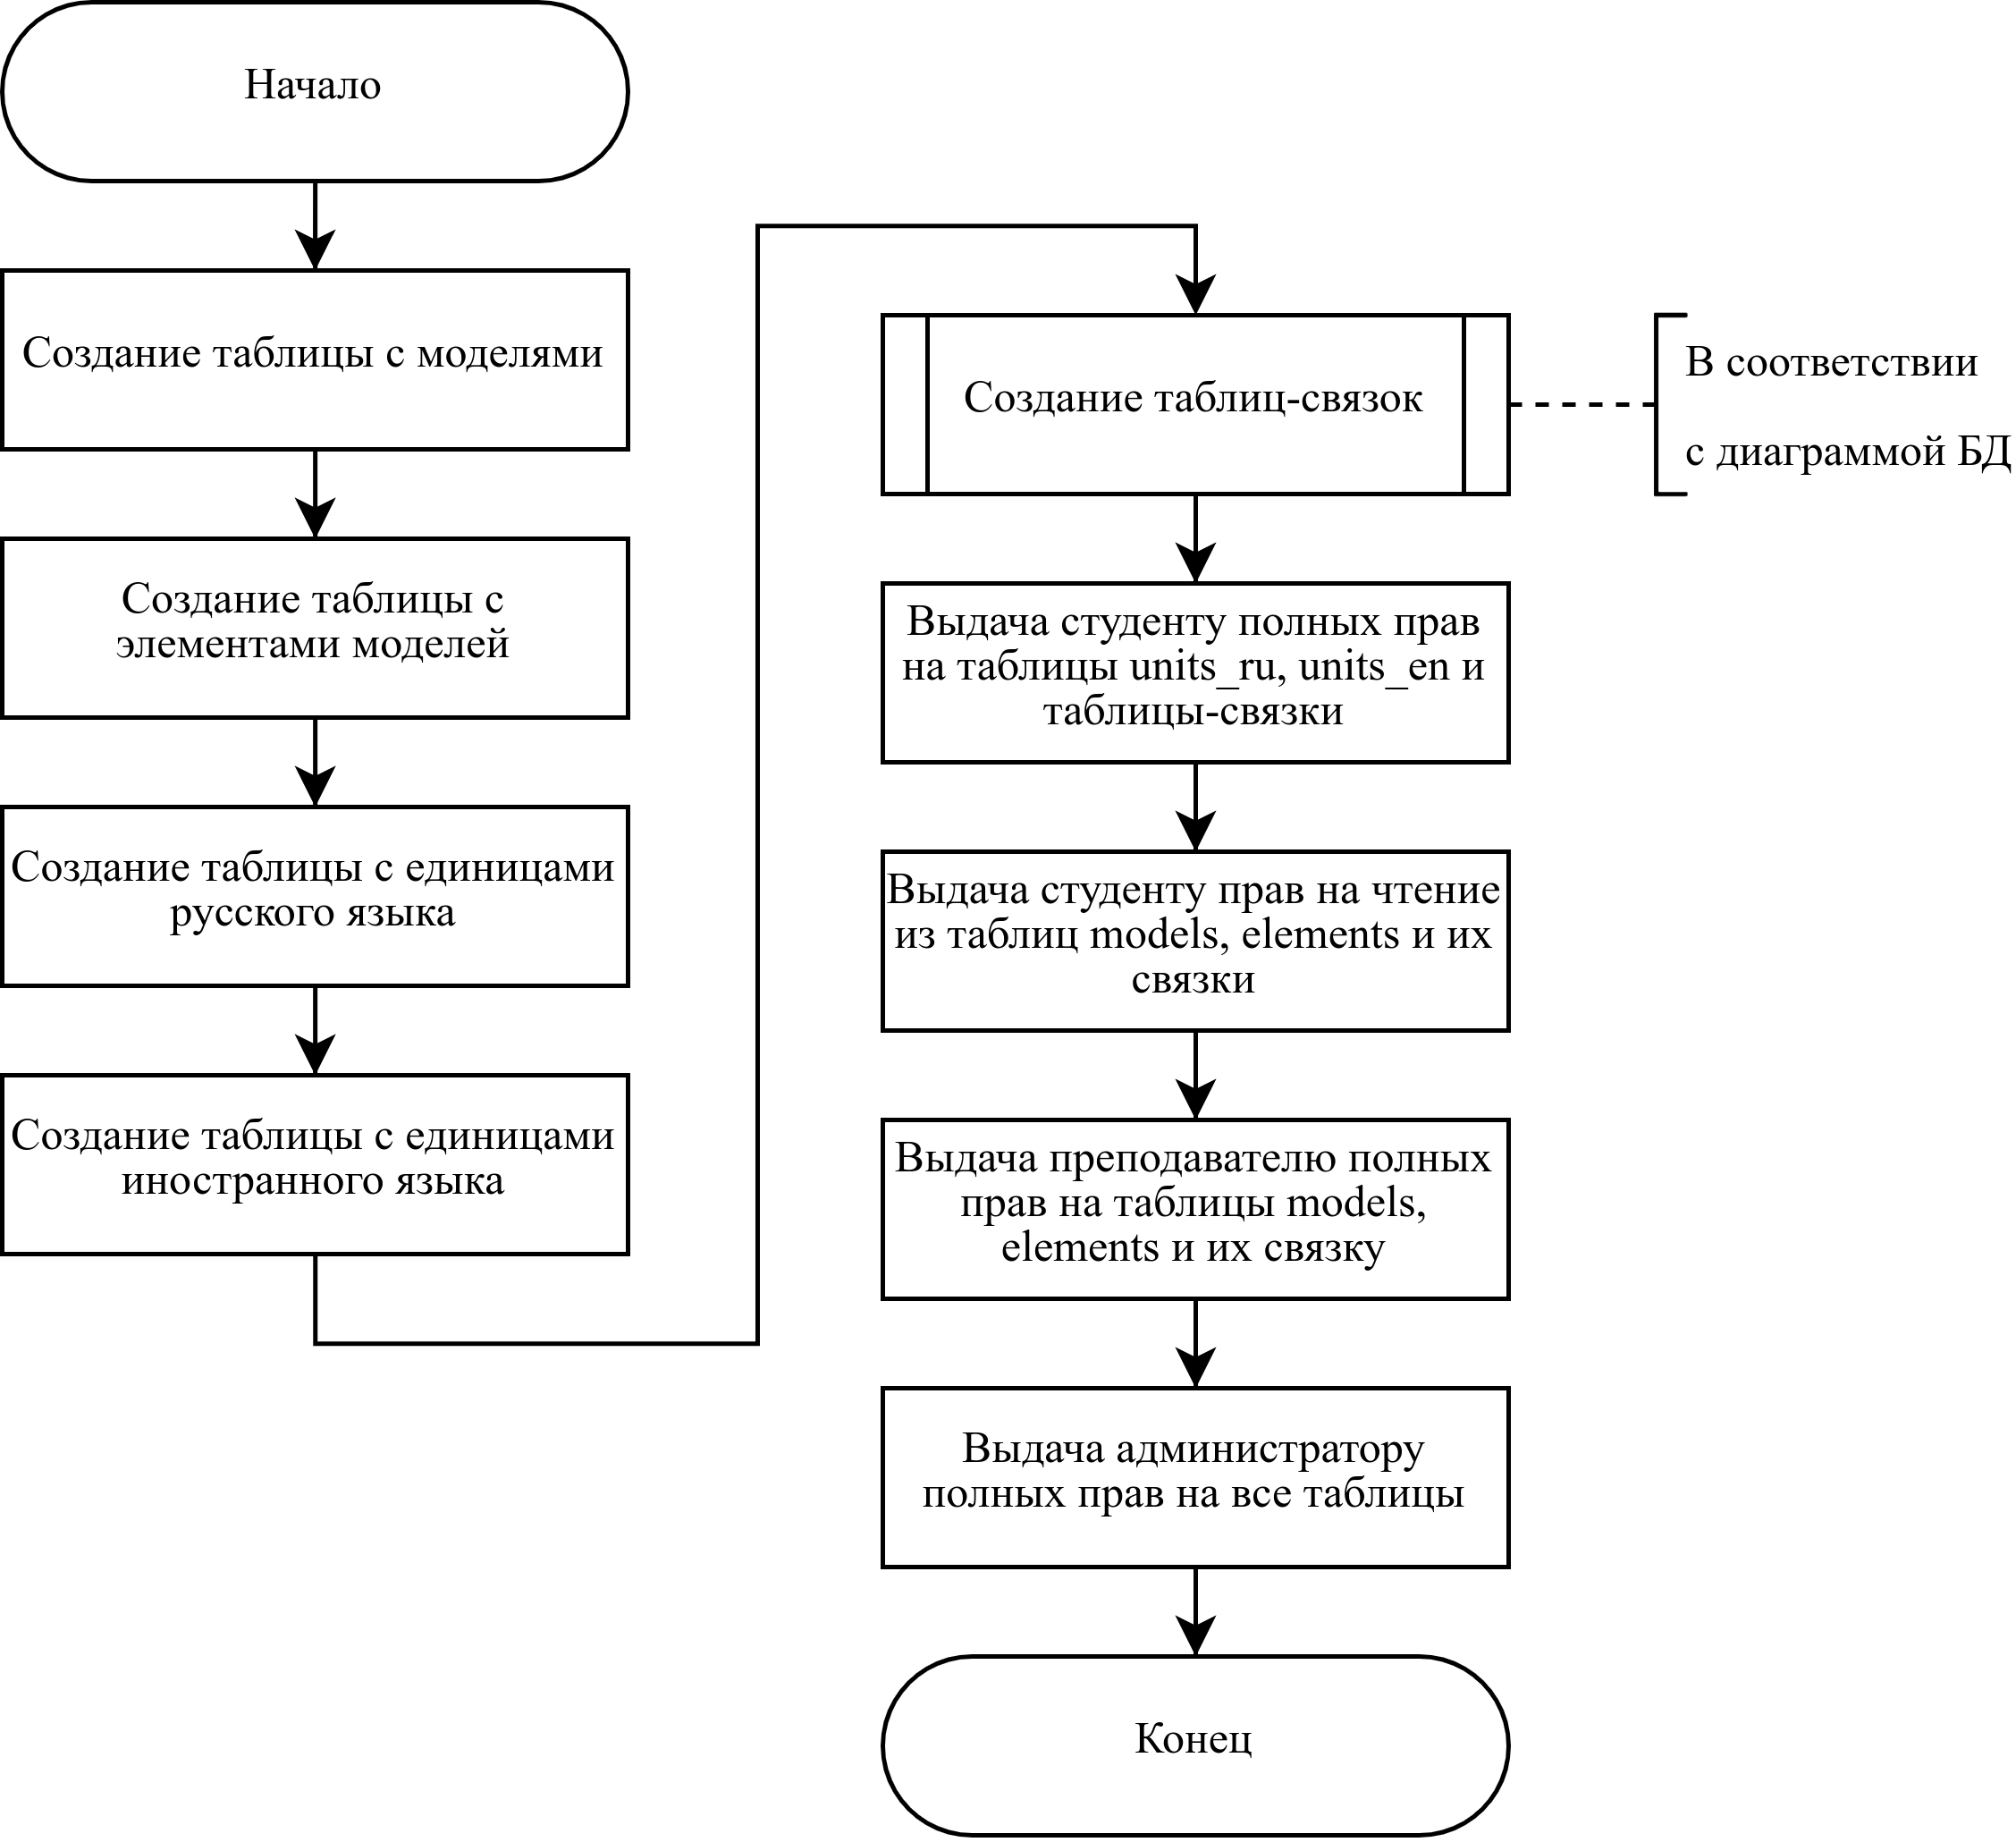
\includegraphics[width=\textwidth ]{img/procedure_algorithm/procedure_algorithm.drawio.png}
	\caption{Схема алгоритма добавления нового слоя разметки текстов}
	\label{fig:proc_alg}
\end{figure} 

\clearpage

\subsubsection{Ролевая модель}

С какими таблицами (и как) могут работать разные пользователи, имеющие разные роли.



\subsection{Проектирование программного комплекса}

\subsubsection{Бизнес-сценарии}

Для разработки функций приложения необходимо описать его бизнес-логику.
Диаграммы в нотации BPMN, отражающие формализацию бизнес-правил, представлены на рисунках \ref{fig:bpmn1}-\ref{fig:bpmn3}. 

\begin{figure}[h]
	\centering
	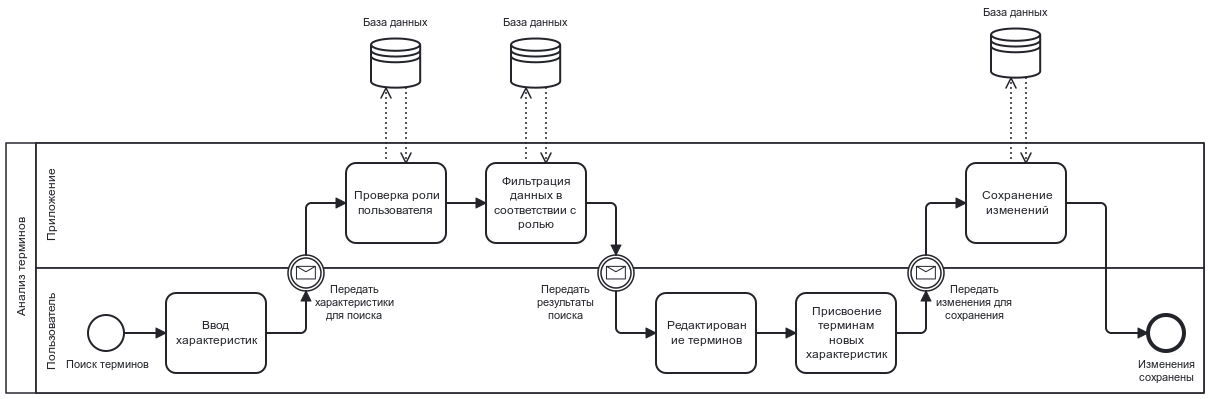
\includegraphics[width=\textwidth ]{img/BPMN/1.png}
	\caption{Авторизация пользователя}
	\label{fig:bpmn1}
\end{figure} 

\begin{figure}[h]
	\centering
	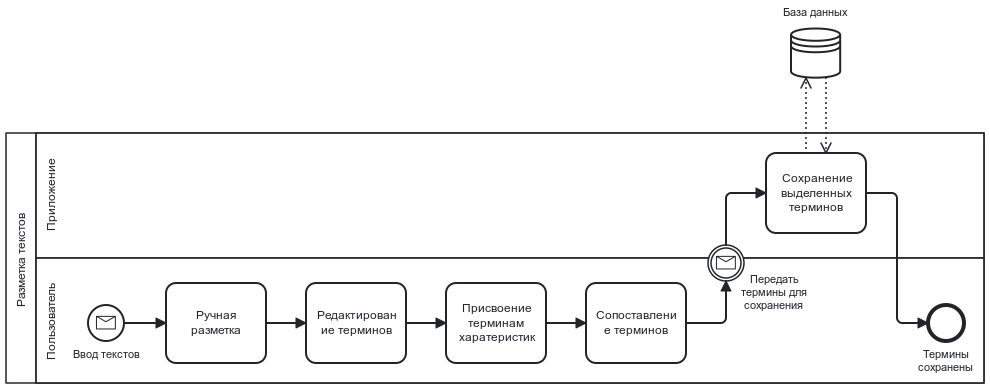
\includegraphics[width=\textwidth ]{img/BPMN/2.png}
	\caption{Разметка текстов}
	\label{fig:bpmn2}
\end{figure} 

\begin{figure}[h]
	\centering
	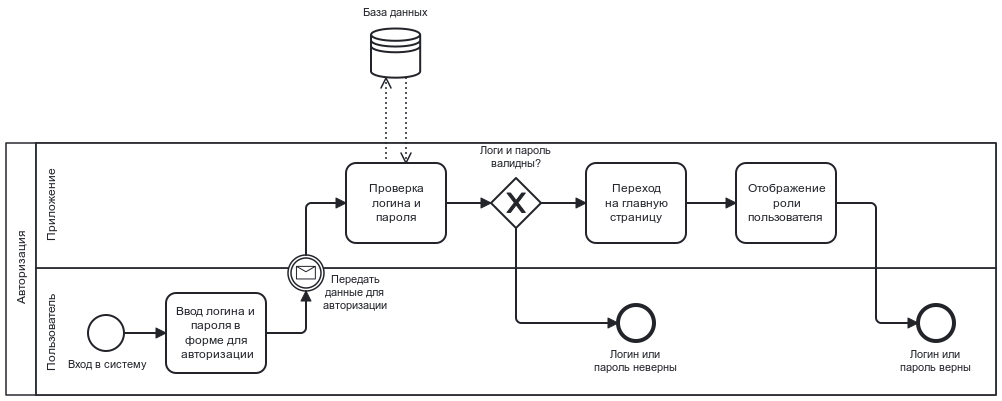
\includegraphics[width=\textwidth ]{img/BPMN/3.png}
	\caption{Анализ терминов}
	\label{fig:bpmn3}
\end{figure} 

\clearpage



\subsubsection{Архитектура приложения}

Приложение состоит из нескольких компонентов: пользовательский интерфейс, базы данных и внешние сервисы. Архитектура приложения определяет, как эти компоненты будут взаимодействовать друг с другом, а также устанавливает границы между разными частями приложения и их ответственностями.

\subsubsubsection{Монолитная архитектура}

Монолитная архитектура --- это традиционная модель программного обеспечения, которая представляет собой единый модуль, работающий автономно и независимо от других приложений. 
% Монолитом часто называют нечто большое и неповоротливое, и эти два слова хорошо описывают монолитную архитектуру для проектирования ПО. 
Монолитная архитектура представляет собой вычислительную сеть с единой базой кода, в которой объединены все бизнес-задачи. Чтобы внести изменения в такое приложение, необходимо обновить весь стек через базу кода, а также создать и развернуть обновленную версию интерфейса, находящегося на стороне службы. Это ограничивает работу с обновлениями и требует много времени.

Монолитную архитектуру можно использовать на начальных этапах проектов, чтобы облегчить развертывание и управление кодом. Это позволяет сразу выпускать всё, что есть в монолитном приложении.

\subsubsubsection{Микросервисная архитектура}

Микросервисная архитектура представляет собой метод организации архитектуры, основанный на ряде независимо развертываемых служб. Эти службы реализуют независимую бизнес-логику и, как правило, имеют собственную базу данных. Обновление, тестирование, развертывание и масштабирование выполняются внутри каждой службы. Микросервисы разбивают крупные задачи, характерные для конкретного бизнеса, на несколько независимых кодовых баз. Микросервисы в составе приложения должны иметь независимую логику и ограниченную зону ответственности.

% Внедрение микросервисов зачастую тесно связано с DevOps, поскольку они лежат в основе методики непрерывной поставки, которая позволяет командам быстро адаптироваться к требованиям пользователей.

При переходе от монолитной архитектуры к микросервисной возникает задача организации взаимодействия компонентов приложения (в частности, транспорта данных). Соответственно, часть проблем переходит из плоскости кода на инфраструктурный и транспортный уровень.

\subsubsubsection{Выбор архитектуры приложения}

Основные преимущества использования монолитной архитектуры:

\begin{enumerate}[label*=\arabic*)]
	\item начальная разработка;
	\item передача данных между компонентами системы;
	\item единая кодовая база; % (нет необходимости строгого соблюдения границ между компонентами системы);
	\item хранение состояния (stateful);
	\item инфраструктура развертывания; %  (один исполняемый файл)
	\item единое версионирование проекта;
	\item производительность; % (чем более тесно связаны компоненты, тем выше производительность системы в целом, так как локальное исполнение эффективнее удалённых вызовов);
	\item интеграционное тестирование;
\end{enumerate}

Основные преимущества использования микросервисной архитектуры:

\begin{enumerate}[label*=\arabic*)]
	\item независимая разработка и выпуск; % (код приложения разбит на несколько кодовых баз, поддерживаемых разными командами разработчиков);
	\item применение разных технологий для каждой выделенной задачи;
	\item независимое развёртывание и горизонтальное масштабирование; % (первое способствует второму)
	\item модульное тестирование; % (протестировать относительно небольшую систему с чётко описанными границами проще, чем большую систему, которая внутри также может взаимодействовать с другими системами); % , т.е. иметь связи с другими элементами
	\item отказоустойчивость системы; % за счёт независимой работы её отдельных компонентов;
	\item повторное использование кода; % (чем меньше внутренних зависимостей, тем проще повторно использовать код);
	\item возможность полностью переписать отдельные компоненты приложения; % (в некоторых ситуациях переписать проще, чем доработать);
\end{enumerate}

%\begin{enumerate}[label*=\arabic*)]
%	\item усложение инфраструктуры развертывания; %  (один исполняемый файл)
%	\item понижение производительности (чем более тесно связаны компоненты, тем выше производительность системы в целом, так как локальное исполнение эффективнее удалённых вызовов);
%	\item усложнение интеграционного тестирования;
%	\item задача организации транспорта данных между компонентами системы;
%	\item возрастание сложности разработки;
%	\item работа с версионностью;
%	\item необходимость поддержания границ между компонентами системы;
%	\item сложность хранения состояния в распределённой системе (stateful);
%\end{enumerate}

%Отличительные свойства микросервисов:
%- Микро не обязательно про размер, но про зону ответственности.
%- Самодостаточны, идеальны для горизонтального масштабирования.
%- Разные технологии для разных задач (но крайне нежелательно разводить "зоопарк технологий").
%- Распределенная кодовая база (декомпозиция задач в командной разработке).
%
%Переход на микросервисы повышает отказоустойчивость системы.
%
%Плюсы микросервисного подхода:
%- Независимая разработка.
%- Независимое развёртывание.
%- Независимая масштабируемость.
%- Повторное использование (меньше внутренних зависимостей -> легче повторно использовать код).
%- Проще переписать, чем доработать. 
%- Проще юнит тестирование (протестировать относительно небольшую систему с чётко описанными границами проще, чем большую систему, которая под капотом также может взаимодействовать с другимим системами, т.е. иметь связи с другими элементами).
%
%Минусы микросервисного подхода:
%- Возросшая сложность для тестирования (речь про интеграционное тестирование).
%- Возросшая сложность для разработчиков. 
%- Возросшая сложность для эксплуатации/Devops. 
%- Выше требования к компетенции (учёт версионности и т.д.). 
%
%По сути все минусы исходят из того, что при переходе от монолита к микросервисам возникает задача организации их взаимодействия (транспорта данных).
%
%Ещё особенности (по сути ещё минусы):
%- Удаленные вызовы дороже локального исполнения.
%- Реальные системы обычно не имеют чётко определённых границ. %%%%%%%%%%%%%%%%%%%%%%%%%%%%%%%%%%%%5
%- Сложности stateful. 
%- Версионность и работа с ней. 
%- Сложности взаимодействия между сервисами. 
%- Распределенные транзакции. %%%%%%%%%%%%%%%%%%%%%%
%- Попытка замаскировать монолит. %%%%%%%%%%%%%%%%%%%%



Для решения поставленной задачи будет использоваться микросервисная архитектура, так как она позволяет независимо разрабатывать и масштабировать компоненты приложения. 
% на самом деле мы здесь выигрываем от большнго количества плюсов...



\subsubsection{Связь компонентов приложения}

%API, или интерфейсы прикладного программирования, предоставляют правила и определения, которые позволяют приложениям общаться и взаимодействовать друг с другом. API определяет типы вызовов и запросов, которые одно приложение может делать другому, способ выполнения этих запросов, используемые форматы данных и соглашения, которым должны следовать клиенты. 
%
%По сути, API-интерфейсы позволяют использовать приложения в более крупных системах, соединяя несколько функций. Функции могут работать и взаимодействовать друг с другом, и вы можете добавлять все больше и больше функций или микросервисов.
%
%Микросервисы могут работать вместе, даже если они написаны на разных языках программирования и работают на разных платформах. По самой своей природе API-интерфейсы предназначены для совместимости. Они создают необходимую связь между микросервисами. Вы можете узнать больше о создании собственных API с помощью DreamFactory .
%
%Понимание архитектурных стилей в API
%REST API и gRPC API относятся к разным архитектурным стилям для создания API. Хотя они подключают микросервисы или приложения, у них есть разные способы сделать это.
%
%Каждый архитектурный стиль предназначен для работы в конкретных случаях, поэтому вам нужно будет принять решение, исходя из ваших потребностей.



Программные компоненты приложения могут взаимодействовать друг с другом с помощью интерфейсов прикладного программирования (Application Programming Interface, API). % , которые действуют как посредники. 
% API отвечает за отправку запроса пользователя в систему, которая затем получает ответ от системы.
API описывает, как выполнять клиентские запросы, какие структуры данных использовать и каких стандартов должны придерживаться клиенты. В нем также описываются виды запросов, которые один компонент может отправлять другому. Для разработки API широко используются архитектурные стили REST API и gRPC.



\subsubsubsection{REST API}

%REST — наиболее часто используемый архитектурный стиль для создания API. Это особенно полезно для веб-приложений и инфраструктур на основе микросервисов.
%
%API-интерфейсы REST используют JSON — текстовый, удобочитаемый формат, который хорошо работает на разных платформах. Хотя это не единственный формат, который можно использовать с REST API, он чаще всего используется из-за своей простоты.
%
%JSON используется для улучшения связи между микросервисами и интернет-приложениями, помогая им взаимодействовать друг с другом. Это наиболее часто используемые случаи для REST API, и вы найдете их повсюду. REST может использовать JSON для получения и отправки сообщений между микросервисами по мере необходимости.

REST, representational state transfer (англ. передача репрезентативного состояния) описывает архитектуру клиент-сервер, в которой данные сервера становятся доступными для клиентов через формат обмена сообщениями JSON или XML. % API квалифицируется как «RESTful», если он соответствует следующим ограничениям:

REST определяется следующими архитектурными ограничениями.

\begin{enumerate}[label*=\arabic*.]
	\item Модель клиент-сервер.
	\item Отсутствие хранения состояния клиента на сервере.
	\item Кеширование ответов сервера на стороне клиента.
	\item Унифицированный интерфейс.
	\item Многоуровневая система. % (на каждом уровне свои ограничения).
	\item Код по запросу (необязательное ограничение).
\end{enumerate}

%Единый интерфейс: API должен предоставлять определенные ресурсы приложения потребителям API.
%Независимость клиент-сервер: клиент и сервер работают независимо. Клиент будет знать только те URI, которые указывают на ресурсы приложения. Обычно они публикуются в документации API.
%Без сохранения состояния: сервер не сохраняет никаких данных, относящихся к запросу клиента. Клиент сохраняет эти «данные состояния» на своем конце (через кеш).
%Кэшируемый: Ресурсы приложения, предоставляемые API, должны быть кешируемыми.
%Многоуровневая: Архитектура многоуровневая, что позволяет поддерживать разные компоненты на разных серверах.
%Код по требованию (COD): это единственное необязательное ограничение REST. Это позволяет клиенту получать исполняемый код сервера в качестве ответа. Другими словами, сервер определяет, как выполняются конкретные действия.



%Он имеет согласованный интерфейс и предоставляет определенные ресурсы приложения для клиентов API.
%Сервер и клиент работают отдельно и независимо. Клиенту будут известны только URI, указывающие на компоненты приложения.
%Это без гражданства. Это означает, что только клиент сохраняет любую информацию о состоянии. Сервер не будет сохранять данные о состоянии клиентского запроса.
%Ресурсы приложения, предоставляемые API, должны быть кэшируемыми.
%Он имеет многоуровневую архитектуру.

% Это применение современных архитектурных решений, которые зависят от нескольких ограничений, позволяющих передавать данные в сетях гипермедиа. Веб-API RESTful требует аргументов в кодировке URL для подключения к службам с использованием протоколов HTTP.RESTAPI-интерфейсы широко используются в современном веб-дизайне для создания расширяемых и надежных API без сохранения состояния.


Приложение, соответствующее данным архитектурным ограничениям, квалифицируется как <<RESTful>>. Это сеть веб-страниц (виртуальная машина), по которой пользователь перемещается с помощью ссылок (переходы состояний) и в результате попадает на нужную страницу (демонстрация состояния приложения).

Также важно отметить, что REST API практически всегда использует протокол HTTP. Это наиболее распространенный формат, используемый для разработки веб-приложений или соединения микросервисов. Если веб-приложение реализует REST API, то клиенты могут использовать каждый его компонент в качестве ресурса. Обычно ресурсы доступны через общий интерфейс, который реализует различные HTTP-методы, такие как GET, POST, DELETE и PUT.

% Каждый компонент, объединяющий микросервисную систему, может отображаться пользователю или заказчику как актив, когдаRESTAPI сделан общедоступным. Этот ресурс можно запросить с помощью HTTPGET,POST,PUTиDELETE команды.

\begin{figure}[h]
	\centering
	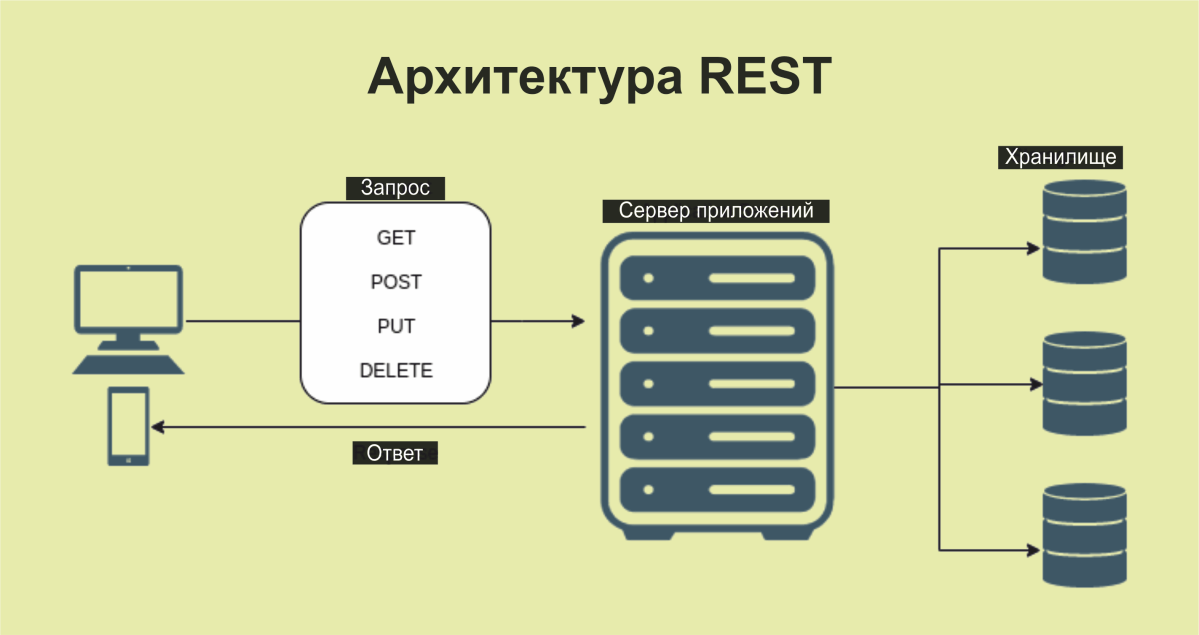
\includegraphics[width=\textwidth ]{img/REST.png}
	\caption{Модель REST API}
	\label{fig:REST}
\end{figure} 

В RESTful API пользователь отправляет запрос на URL-адрес --- унифицированный указатель ресурсов, который вызывает ответ с полезной нагрузкой в JSON, XML или любой другой поддерживаемый формат данных. Полезная нагрузка представляет собой ресурс, который нужен пользователю. Общие запросы клиентов включают

\begin{itemize}[label*=---]
	\item HTTP-метод, указывающий, что должно обрабатываться на ресурсе;
	\item путь к ресурсу;
	\item заголовок с данными о запросе;
	\item полезная нагрузка сообщения для конкретного клиента.
	
\end{itemize}

% В поле Accept заголовка пользователь указывает типы данных, которые он может принимать. Заголовок типа содержимого, который идентифицирует формат доставки сообщения, используемый в теле ответа, отправляется сервером API вместе с полезными данными, которые он доставляет пользователю, выполняющему запрос. Код ответа, который информирует пользователя о статусе результата вызова API, также включается в тело ответа.





\subsubsubsection{gRPC}

%Крупномасштабное развертывание gRPC обычно имеет несколько идентичных серверных экземпляров и несколько клиентов. Каждый сервер имеет определенную мощность. Балансировка нагрузки используется для оптимального распределения нагрузки от клиентов между доступными серверами.

gRPC, remote procedure call (англ. удалённый вызов процедур) --- это протокол RPC, реализованный поверх HTTP/2 (протокол прикладного уровня). 
% HTTP/2 — это протокол уровня 7 (прикладной уровень), который работает поверх протокола TCP (уровень 4 — транспортный уровень), который работает поверх протокола IP (уровень 3 — сетевой уровень). gRPC имеет много преимуществ по сравнению с традиционными механизмами HTTP/REST/JSON, такими как
Основные особенности gRPC:

\begin{itemize}[label*=---]
	\item бинарный протокол (HTTP/2);
	\item мультиплексирование множества запросов на одно соединение (HTTP/2);
	\item сжатие заголовков (HTTP/2);
	\item строго типизированный сервис и определение сообщения (Protobuf);
	\item идиоматические реализации библиотек клиент/сервер на многих языках (Golang, C++, Python и другие);
	\item интеграция с такими компонентами экосистемы, как обнаружение сервисов, преобразователь имен, балансировщик нагрузки, трассировка и мониторинг и другие.

\end{itemize}

% Как архитектура RPC с открытым исходным кодом, gRPC создает высокоскоростную связь между микросервисами. Первоначально он был разработан Google для улучшения связи.

Удаленный вызов процедур --- это веб-архитектура, позволяющая выполнять запросы на сервере с использованием предопределенных форматов сообщений. При этом сервер может быть как локальным, так и удалённым.

\begin{figure}[h]
	\centering
	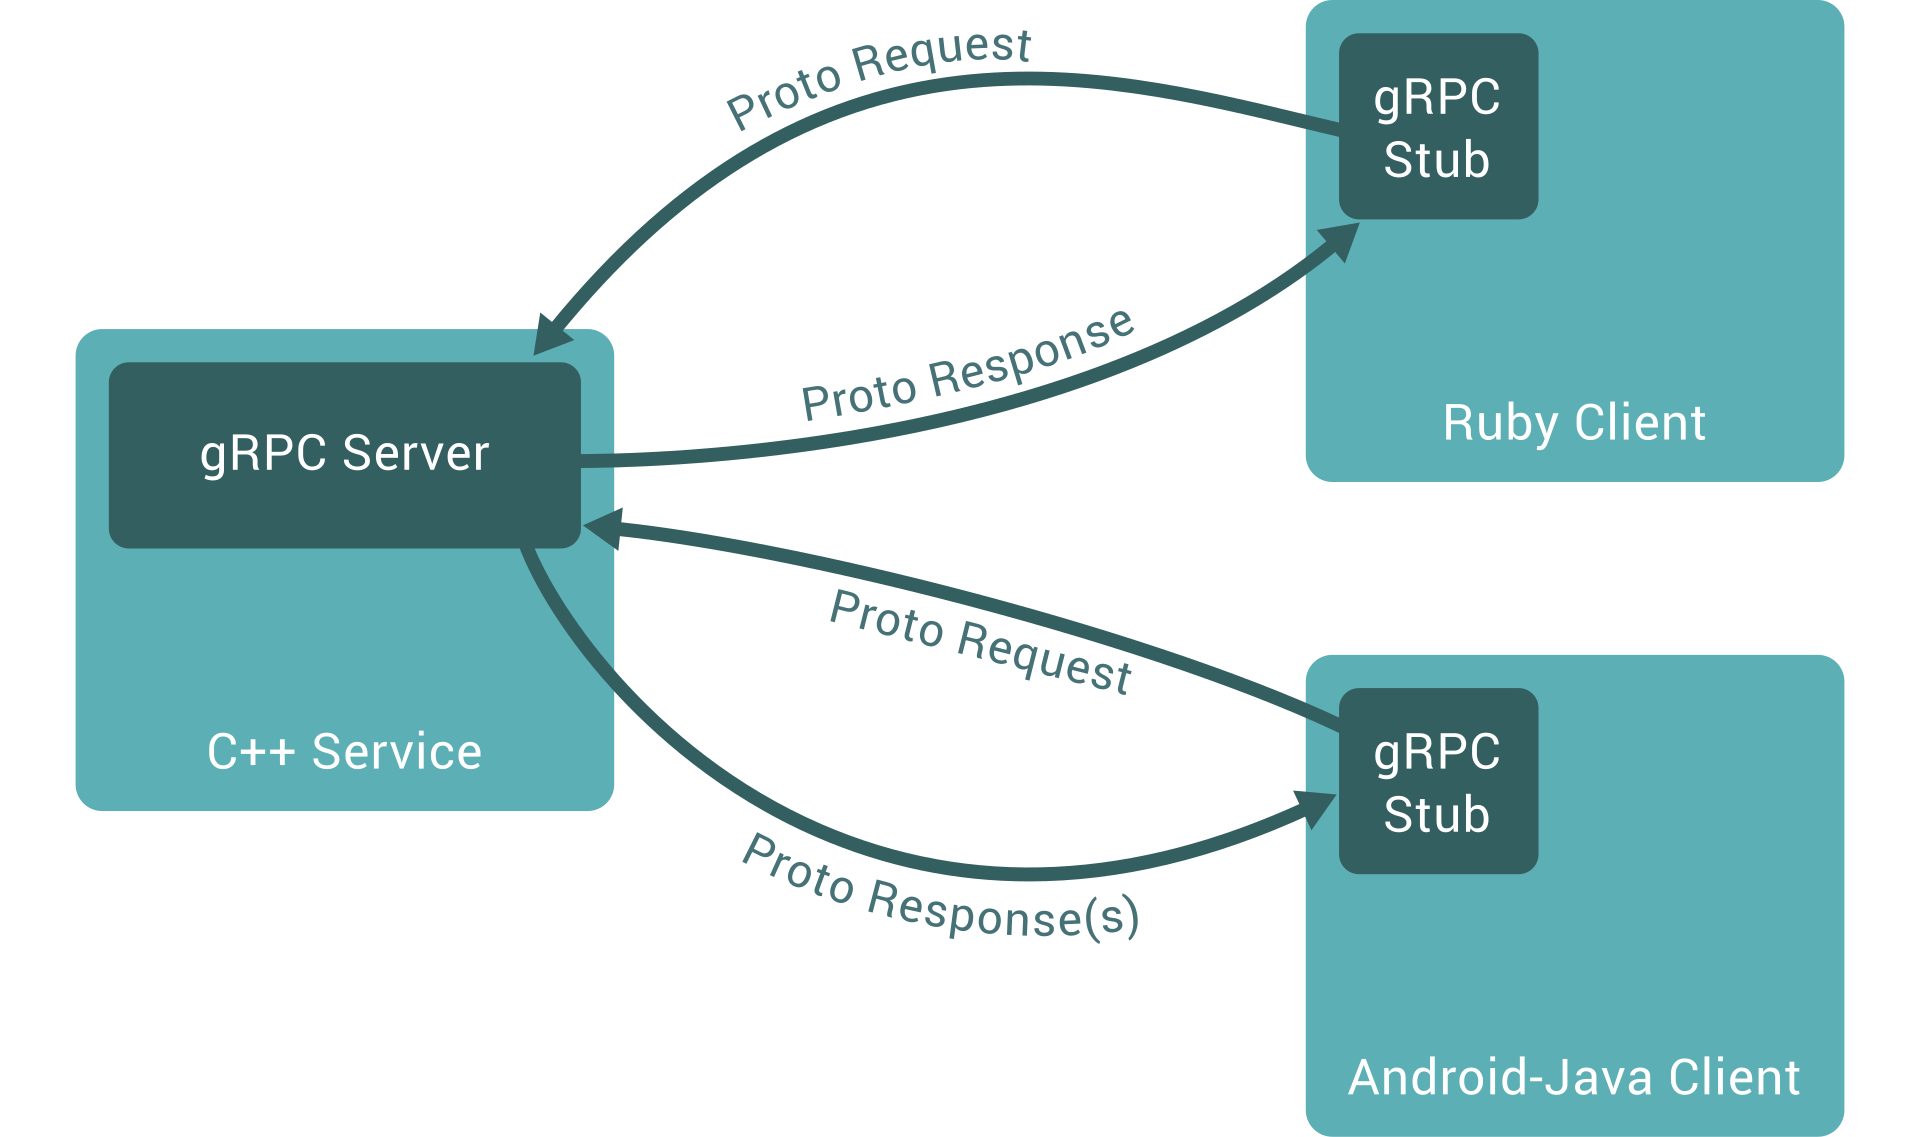
\includegraphics[width=\textwidth ]{img/gRPC.png}
	\caption{Модель gRPC}
	\label{fig:gRPC}
\end{figure} 

Эта архитектура API позволяет нескольким функциям, созданным на разных языках программирования, работать вместе благодаря API. gRPC использует формат обмена сообщениями Protobuf (англ. буферы протокола), который используется для сериализации структурированных данных. Для определенного круга задач API gRPC является более эффективной альтернативой REST API.



\subsubsubsection{Выбор взаимодействия компонентов приложения}

В таблице \ref{tbl:compare} представлено сравнение gRPC и REST API.

\clearpage
\begin{table}[h]
	\begin{center}
		\captionsetup{justification=RaggedRight, singlelinecheck=off}
		\caption{Сравнительная характеристика gRPC и REST API}
		\label{tbl:compare}
		\begin{tabular}{|l|l|l|}
			\hline
			Характеристика & gRPC & REST API \\
			\hline
			Формат & Унарные двусторонние & Только клиентские запросы \\
			коммуникации & запросы или потоковая & \\
			 & передача & \\
			\hline
			Способ & RPC & HTTP-методы \\
			коммуникации & & \\
			\hline
			Протокол & HTTP/2 & HTTP 1.1 \\
			\hline
			Формат сообщений & Protobuf (protocol buffers) & JSON/XML \\
			\hline
			Генерация кода & С помощью компилятора & Сторонние решения, \\
			& Protobuf & такие как Swagger \\
			\hline
		\end{tabular}
	\end{center}
\end{table}

Для решения поставленной задачи будет использоваться REST API по следующим причинам:

\begin{enumerate}[label*=\arabic*.]
	\item Универсальность: позволяет связывать любые сервисы, которые могут принимать или отправлять HTTP-запросы.
	\item Скорость развёртывания.
	\item Поддержка инструментов описания API (Swagger, ReDoc, Apiary и другие).
	
\end{enumerate}

% gRPC, потому что между сервисами передаётся много данных (структуры, представляющие очень большие тексты), поэтому критически важен быстрый транспорт.



\subsubsection{Структура программного комплекса}

На рисунке ????? представлена структура программного комплекса, оформленная в виде диаграммы развёртывания. Она отражает компоненты системы и способы их взаимодействия. 

Обязательно здесь упомянуть про контейнеризацию и Docker!



% \subsubsection{Диаграммы последовательностей}



\subsubsection{Паттерны проектирования}

Паттерны проектирования повышают степень повторного использования проектных и архитектурных решений. Они помогают выбрать альтернативные решения, упрощающие повторное использование системы, и избежать тех альтернатив, которые его затрудняют. Паттерны улучшают качество документации и сопровождения существующих систем, поскольку они позволяют явно описать взаимодействия классов и объектов, а также причины, по которым система была построена так, а не иначе \cite{patterns}.

Далее будут описаны паттерны проектирования, которые будут использованы при разработке программного комплекса.

% \subsubsubsection{Active Record}

\subsubsubsection{Repository}

Repository (репозиторий) \cite{repository_pattern} --- это слой абстракции, инкапсулирующий в себе всё, что относится к способу хранения данных. Он предназначен для отделения бизнес-логики от деталей реализации слоя доступа к данным.

Паттерн Репозиторий стал популярным благодаря DDD (Domain Driven Design). В отличие от Database Driven Design, в DDD разработка начинается с проектирования бизнес логики, причём во внимание принимаются только особенности предметной области, а всё, что связано с особенностями хранения данных, игнорируется.

Применение данного паттерна не предполагает создание только одного объекта репозитория во всем приложении. Хорошей практикой считается создание отдельных репозиториев для каждого бизнес-объекта или контекста, например: OrdersRepository, UsersRepository, AdminRepository.

Репозиторий --- это высокоуровневая абстракция доступа к данным. Интерфейс каждого конкретного репозитория определяется в слое бизнес-логики наряду с классами предметной области. Реализация каждого репозитория находится в слое доступа к данным (Data Access Layer, DAL), который состоит из реализации каждого репозитория, ORM-специфичных классов, сущностей, классов-сопоставлений (mapping), контекстов данных и т.д.

\subsubsubsection{Dependency injection}

% В терминах объектно-ориентированной разработки программного обеспечения это означает следующее: взаимодействующие классы должны полагаться на инфраструктуру) для предоставления необходимые услуги.

Dependency injection (инъекция зависимостей) \cite{dependency_injection} --- это набор принципов и паттернов проектирования программного обеспечения, который позволяет разрабатывать свободно связанный код.

В программной инженерии внедрение зависимостей --- это техника, при которой один объект предоставляет зависимости другому объекту. Зависимость --- это объект, который может быть использован, например, в качестве сервиса. Вместо того чтобы клиент указывал, какой сервис он будет использовать, что-то указывает клиенту, какой сервис использовать. Инъекция относится к передаче зависимости (сервиса) в объект (клиент), который будет его использовать. Сервис становится частью состояния клиента. Передача сервиса клиенту, вместо того чтобы позволить клиенту создать или найти сервис, является фундаментальным требованием паттерна.

Создание объектов непосредственно в классе является негибким, поскольку фиксирует класс на определенных объектах и делает невозможным дальнейшее изменение инстанцирования независимо от класса. Это не позволяет классу быть многократно используемым, если потребуются другие объекты, и затрудняет тестирование класса, поскольку реальные объекты не могут быть заменены имитационными объектами.

Зависимость от интерфейса является более гибкой, чем зависимость от конкретных классов. Объектно-ориентированные языки предоставляют способы, с помощью которых можно заменить эти абстракции конкретными реализациями во время выполнения. Инъекция зависимостей помогает кодовую базу гибкой и пригодной для повторного использования.



\subsubsubsection{Template method}

Template Method (шаблонный метод) \cite{patterns} --- паттерн поведения классов.

Шаблонный метод определяет скелет алгоритма, перекладывая ответственность за некоторые его шаги на подклассы. Это позволяет подклассам переопределять отдельные шаги алгоритма, не меняя его общей структуры.

Основные условия для применения паттерна шаблонный метод:

\begin{itemize}[label*=---]
	\item однократное использование инвариантных частей алгоритма, при этом реализация изменяющегося поведения остается на усмотрение подклассов;
	\item необходимость вычленить и локализовать в одном классе поведение, общее для всех подклассов, чтобы избежать дублирования кода;
	\item управление расширениями подклассов (шаблонный метод можно определить так, что он будет вызывать операции-зацепки (hooks) в определенных точках, разрешив тем самым расширение только в этих точках);
\end{itemize}

Шаблонные методы --- один из фундаментальных приемов повторного использования кода. Они играют особенно важную роль в библиотеках классов, поскольку предоставляют возможность вынести общее поведение в библиотечные классы. Шаблонные методы приводят к инвертированной структуре кода, которая подразумевает, что родительский класс вызывает операции подкласса, а не наоборот.

\pagebreak